% !TEX root = SystemTemplate.tex

\chapter{User Documentation}

%This section should contain the basis for any end user documentation for the system. 
 %End user documentation would cover the basic steps for setup and use of the system. 
 %It is likely that the majority of this section would be present in its own document 
%to be delivered to the end user.  However, it is recommended the original is contained 
%and maintained in this document. 

%\newpage   %% 
%%  The user guide can be an external document which is included here if necessary ...
%%  a single source is the way to go.

\section{User Guide}

%The source for the user guide can go here.    You have some options for how to handle the user docs.  If you have some {\tt newpage} commands around the %guide then you can just print out those pages.   If a different formatting is required, then have the source in a separate file {\tt userguide.tex} and include %that file here.  That file can also be included into a driver (like the senior design template) which has the client specified formatting.  Again, this is a single %source approach.   

To use this testing program:
  
 1) make sure that you are in the directory where the program is installed. This should also be the directory which you wish to run the test suite in.
 
 2) Compile the program using the makefile (simply type makefile).
 
 The directory should be the full file path to the proper directory.
 
 Do not put parenthesis around the directory path.
 
 3) The last step will have generated an executable file which may be run by typing ./<executableName>.
 
 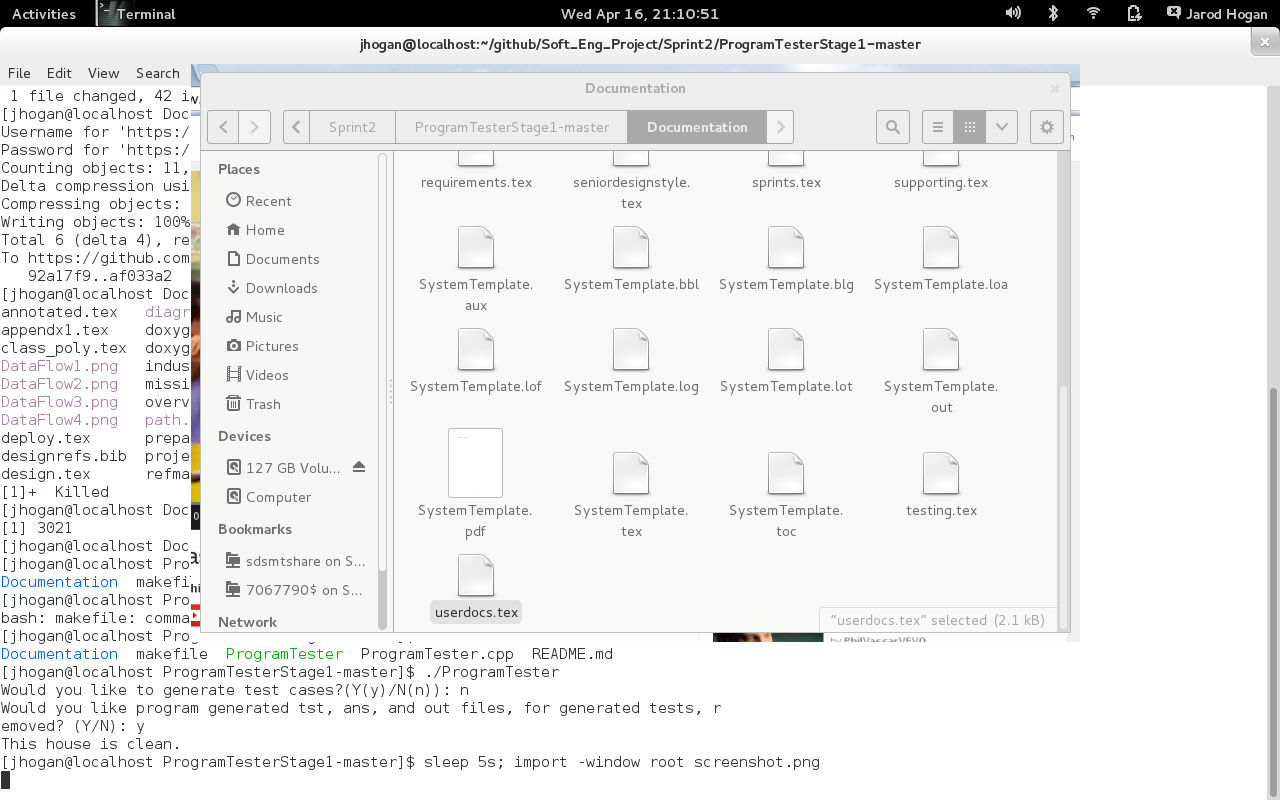
\includegraphics[width=0.75\textwidth]{./screenshot}
 
This program is ment to be used with a Linux system.

%% \newpage  %%  if needed ...
\section{Installation Guide}
Insure that ProgramTester.cpp and makefile are in the same
 directory and just type "make" on the command line to install the program
 
 Alternatively you may just compile on the command line with:
 
 g++ ProgramTester.cpp -o tester
  
 Both of these require that you have g++ installed on your system.
 The program is meant to be used on a Linux system.

%% \newpage  %%  if needed ...
%\section{Programmer Manual}

